%!TEX root = article.tex

\section{Introduction}
\label{s:Introduction}

\subsection{Motivation}
%Why do we do this at all ?

This thesis aims to understand and specify how blood flow and oxygen transport has been simulated until today. The goal is to see how far existing methods, especially the Green's Function Method applied to this field by Secomb et al. \cite{Secomb2004} can produce accurate results for new and especially complex networks. A new model using an open source software called $DuMu^x$ \cite{flemischdumux} was implemented to offer a different approach for oxygen transport and diffusion simulations.

\subsection{Structure of the Thesis}
%This thesis will have following structure ...

First, a short insight to the physiological background of blood flow and oxygen transport in the body will be given.The general process of oxygen delivery to the tissue and oxygen consumption by the tissue will be explained. The main subject will be the transport of oxygen in the body, starting in the blood flow and ending in the diffusion into the tissue through a general diffusion process.
\\The results of oxygen transport simulation methods, especially the Green's Function Method, will later be discussed and evaluated for different networks. In addition to this, a new oxygen delivery model was implemented using an open source software called $DuMu^x$. The focus of this thesis is to understand when and why the Green's Function Method produces physiologically accurate results, how it can perform on new networks and compare these results to alternatives such as the implemented method on $DuMu^x$.

\section{Blood Flow and Oxygen Delivery}
%How does this work physiologically ?

In this section the physiological aspects will be discussed, and the main goal of computations and simulations in this field will be explained. This part is mainly about the physiological points in blood flow and oxygen transport, as well as oxygen consumption in tissue and further outlook in this field. (i.e. EPO and tumor oxygen delivery etc.)
\\Blood is pumped through the heart into the whole body. This results in pressure gradients, accelerating the fluid through the arteries.
\\In this thesis, the flow and transport through micro-vessels in the capillary range is the main concern, where generally the time-dependency of the velocity of blood will be neglected. We use a steady-state approximation for the flow rate, and thus assume a constant velocity. This means that there is no variation of velocity depending on time for any given point in the network.

\subsection{Blood Flow}
%Purely physiological Blood Flow part (with mathematical formulas to describe processes)
%Discuss General Hemodynamics

Blood flow in the body can be approximated by the Navier-Stokes equations.
\\But rather talk about purely physiological things first.
\\Put some papers and references in and explain some values and parameters.
\\Use mathematics paper for blood flow calculations \cite{rahman2012mathematical}.
\\Papers to cite: \cite{pittman2011regulation}
\\
\\

\subsection{Oxygen Transport and Delivery}
%Purely physiological Oxygen part (with mathematical formulas to describe processes)

How does this oxygen related stuff physically and physiologically work ?
\\Again put some papers and references in and explain some physical diffusion equations, values and parameters.
\\Why do we care about this etc. ?
\\Diffusion, Parameters, etc. etc.
\\Use Vasomotion paper for oxygen delivery \cite{goldman2001computational}

\subsubsection*{Oxygen Transport in the Blood}
%Transport with the flow
%Binding of Oxygen to Red Blood Cells
%Oxygen Concentration etc.

-Plasma and Red Blood Cells
\\-Hemoglobin
\\-Myoglobin
\\Blood is basically composed of two phases: liquid and cells, which is the plasma and the red blood cells. The red blood cells build nearly half of the total blood volume, and are the main carriers of oxygen in the blood \cite{pittman2011regulation}.
\\Papers to cite: \cite{hellums1977resistance}.

\subsubsection*{Oxygen Diffusion Into the Tissue}
%Diffusion out of the Vessels
%Diffusion Process - Transport in the Tissue
%Delivery of Oxygen to the Cells

-What is Diffusion ?
\\-Fick's Law of Diffusion and Concentration Gradients
\\-Diffusion Properties and some general Parameters
\\Papers to cite: \cite{hellums1977resistance}, \cite{fletcher1980facilitated}
\\

\subsection{Current Trends in Modeling}
%Use a few papers to give examples for previous and actual approaches

Do link to modeling and models in this field in general, then link this to computational models in this field and their use. Actual trends and what people hope for in the future (in terms of computational power, computational methods but also from a medical perspective) is also interesting.
\\In order to simulate flows, Computational Fluid Dynamics (CFD) is a tool that can be used to produce results which can not be obtained through in vitro or in vivo experiments. For this reason and because the computational capabilities available are growing everyday, modeling and simulating processes in the body is taking an increasingly important role in biological and medical sciences.
\\In our case, the focus will lie on oxygen transport simulations and their computational implementation.\\
\\Generally Blood Flow in the body can be approximated by the Navier-Stokes equations. The Transport of oxygen in the Blood can then be linked to this by the Transport Equations. These physical equations are quite straightforward to implement and solve numerically. The next task remains the biggest problem in actual research: Link this transport to the diffusion process out of the vessels and into the tissue. The biggest problems here seem to be in choosing the right/appropriate boundary conditions to get exact results. Also, many numerical methods fail or more specifically become unstable when the vessel network becomes complicated and heterogeneous. There are already good methods to produce results for the Krogh model, but to compute oxygen fields in very complex networks like in the kidney, these models do not provide the desired results.
\\Steady-State approximation for simulations: Need this assumption for Michaelis-Menten relation.
\\Papers to cite: \cite{rahman2012mathematical}, \cite{goldman2001computational}, \cite{kuzmin2010guide}, \cite{lee2017accounting}, \cite{hoofd1992updating}, \cite{beard2001modeling}, \cite{Secomb2004}

%In each of your categories (or subcategories if your topic is
%broad), we would like the following three points to be developed:
%\begin{enumerate}
 %   \item Concepts, definitions, value
%of this topic etc. For explanations that do not really fit in the
%text you may want to use footnotes\footnote{footnotes are shown
%below like this.} or by using the appendix (e.g. "see appendix
%\ref{s:ExtraStuff}").
 %   \item State of the art, discussing the work in the field, etc. E.g. Shaninpoor et al. \cite{shaninpoor98} have shown that ...
 %   \item Outlook: where do you feel this field is going. How would you continue your research on this
  %  topic?
%\end{enumerate}

\section{Simulation Methods}
%Everything about the computations behind the simulations and all I did.

As mentioned previously, this thesis is focussing on the analysis of simulation methods for oxygen transport and the delivery to the tissue surrounding the vessels. In this section I will try to give an overall understanding to the theoretical background to the Green's Function Method and accordingly the code developed by Secomb et al. \cite{Secomb2004}. Later on I will present a new model that I implemented using $DuMu^x$. Both the methods and the produced results will be discussed in the following sections.

\subsection{Green's Function Method Code}
%Here I will talk about everything concerning the Green's Method Code.

The Green's Function Method was first used for numerical computations of oxygen delivery in the tissue by Secomb et al. \cite{Secomb2004}. It can deliver accurate results with lower computational cost, due to the fact that the number of unknowns is reduced. For simple networks like the examples specified in the next chapter, the method seems to be stable and produce accurate results. However, using new and more complex networks, the Green's Function Method seems to produce bad results and shows characteristics of unstability (at least we think so for now). Obviously as the results get bad, the computational advantages of this method are not of any use (bad formulation?).
\\The mathematical background behind the Green's Function Method and the numerical method derived from it will be discussed in the upcoming section. The accuracy of produced results as well as the physiological meaning behind these results will be the main subject in this chapter.

\subsubsection{Green's Function Model}
%Just mathematical theory behind this method

General explanation about Green's Method code and how it works, especially mathematics behind the Green's Function Method (many mathematical formulas) and why it makes sense to use this. Also especially why is this interesting in physiological applications and oxygen delivery/consumption simulations ?
\\Goals:
\\- Avoid no flux boundary condition
\\- Find a systematic method that can be applied to tissue domains of arbitrary shape
\\- Find a cheap solution in terms of computational cost (when compared to implicit methods)
\\- Green's function method is computationally less expensive than implicit methods, due to the fact that there is a lower number of unknowns

\subsubsection*{The Computational Model}
%Methods and physiological assumptions used in this model.
%Very useful to use Governing Equations section of Secomb here

In this subsection, the used physical quantities, the assumptions and governing equations will briefly be explained. The equations cited here are, in my opinion, the most important ones to describe the physical background for the treated problem. This part strongly relies on the description by Secomb et al. \cite{Secomb2004}.
\\When looking at the code of the Green's Function Method, and especially at the inputs \ref{Inputs}, one can see that the tissue is modeled as a homogeneous medium. This results in constant oxygen diffusivity and solubility coefficients D and $\alpha$ respectively. These quantities usually have to be specified in the SoluteParams.dat-file. A more detailed explanation to the Inputs can be found in the Inputs section \ref{Inputs}.
\\The governing equations are listed here, with a short explanation for each of them:
\\As previously described, diffusion will play an important role in oxygen transport in the body, as oxygen is reaching the tissue by diffusing out of the vessels. This physical phenomenon is described by Fick's Law of Diffusion:
\begin{equation}
\\J = - D \frac{dc}{dx}
\label{Fick}
\end{equation}
%
Where J is the diffusive flux, D is the previously mentioned diffusivity coefficient, and dc/dx is the derivative of the concentration with respect to the distance x.
\\In addition to this, the principle of conservation of mass applies to oxygen, and we have:
\begin{equation}
\frac{\delta \rho} {\delta t} + \nabla (\rho v) = 0
\end{equation}
%
These two fundamental equations can be combined to finally get:
\begin{equation}
\\D\alpha\nabla^2P = M(P)
\label{eq:DiffusionEq}
\end{equation}
%
\ref{eq:DiffusionEq} describes the dependency between the oxygen partial pressure P and the consumption rate M(P). Here I would like to mention the fact that partial pressure is physically nothing else than the concentration used in \ref{Fick}.
For the consumption, a Michaelis-Menten relationship applied to the problem is used:
\begin{equation}
\\M(P) = \frac{M_0P}{(P_0 + P)}
\label{eq:MichaelisMenten}
\end{equation}
%
In \ref{eq:MichaelisMenten}, M(P) is the consumption, $M_0$ the demand and $P_0$ the partial pressure at half-maximal consumption.
\\As previously mentioned, the second important physical phenomenon to describe our transport problem is the convective transport in the blood flow. To model this, we need to know the rate of convective oxygen that is transported through a single vessel segment.
\begin{equation}
\\f(P_b) = Q(H_DC_0S(P_b) + \alpha_{eff}P_b)
\label{eq:ConvTrans}
\end{equation}
%
In \ref{eq:ConvTrans}, the flow rate of blood is Q, and $H_D$, S, $C_0$, $P_b$ and $\alpha_{eff}$ are parameters such as discharge hematocrit, oxyhemoglobin saturation or partial pressure of oxygen in the blood. (Here specify everything yes or no ? Maybe use a symbols table at beginning to make things easier).
\\The previously mentioned oxyhemoglobin saturation can be computed by Hill's equation:
\begin{equation}
\\S(P_b) = \frac{P_b^n}{(P_b^n+P_{50}^n)}
\label{eq:Hill}
\end{equation}
In Hill's equation \ref{eq:Hill}, $P_b$ ist the previously mentioned partial pressure of oxygen in blood, $P_{50}$ is the partial pressure of oxygen at 50\% saturation and n is a constant.
%
\\Another important equation that we need to describe the given problem is the relationship describing the rate of of diffusive oxygen efflux per unit vessel length:
\begin{equation}
\\ \frac{df(P_b)}{ds} = -q_v(s)
\label{eq:ConsOxygen}
\end{equation}
\ref{eq:ConsOxygen} is obtained by using the conservation of oxygen along a vessel segment.
%
\\The continuity condition for the partial pressure of oxygen on the vessel-tissue interface gives a second equation for the diffusive oxygen flux:
\begin{equation}
\\q_v(s) = -D\alpha \int_{0}^{2\Pi} 
\frac{\delta P}{\delta r}r_v d \Theta
\label{eq:DiffFlux}
\end{equation}
\ref{eq:DiffFlux} is an integral form of the diffusive flux $q_v(s)$.
%
\\The relation between the partial pressure of oxygen in the tissue and the blood can be approximated with the following equation \cite{hellums1977resistance}:
\begin{equation}
\\P_v(s) = P_b(s) - Kq_v(s)
\label{eq:Hellums}
\end{equation}
\ref{eq:Hellums} is the Hellums relationship.
\\Here $P_v(s)$ represents the partial pressure of oxygen averaged around the circumference of the vessel, K is the intravascular resistance to radial oxygen transport, which is assumed to be constant but depends on the vessel diameter. The value for K for each vessel can be found in the input file IntravascRes.dat \ref{Inputs} which has to be given to the code.
%
\\As discussed in the first part, myoglobin is a substance (molecule?) that supports the diffusion of oxygen in the tissue. The effects of myoglobin-facilitated diffusion can sometimes be neglected, when the myoglobin concentration is very low. For the case where the effects of myoglobin are relevant, one can simply replace the partial pressure P with the partial pressure $P^*$, given in the following equation \ref{eq:Myoglob}.
\begin{equation}
\\P^* = P + \frac{D_{Mb}C_{Mb}V_mS_{Mb}(P)}{D \alpha}
\label{eq:Myoglob}
\end{equation}
In \ref{eq:Myoglob}, $D_{Mb}$, $C_{Mb}$, $V_m$ and $S_{Mb}$ are the diffusion coefficient, the concentration, the molar volume and the oxygen saturation of Myoglobin respectively. D and $\alpha$ are the same constants mentioned previously, which were the diffusivity and the solubility coefficients of oxygen.

\subsubsection*{Mathematics Behind Green's Function Method}
%Mathematical Background to this Method. What's so special about it ? Is there any advantage at first sight ?
%Very useful to use Green's Function Formulation section of Secomb here

 Similar to the previous section, this section will strongly rely on \cite{Secomb2004}. In this subsection, the Green's Function Method, its equations and the application to the given problem/field will be explained.
\\In this section, I will focus on giving a good and understandable insight to the Green's Function Method and its specific application, instead of getting lost in details. More specific low-level informations about the code and its implementation will follow later.
\\The main idea of the Green's Function Method approach is to model blood vessels as discrete oxygen sources. The oxygen consumption is then modeled by a set of discrete oxygen sinks. As previously described, our goal is to simulate the oxygen transport to finally obtain the oxygen concentration for every node in our tissue and vessel network. In general terms, the oxygen field is computed by a superposition of the fields resulting from each of the sources and sinks.
\\The strengths of the sources are unknowns in this problem. The sinks are unknowns as well, due to the fact that the oxygen consumption depends on the local partial pressure of oxygen, as one can see in \ref{eq:MichaelisMenten}.
%
\\When defining the Green's Function G as the potential at a point $\textbf{x}$ and putting this potential equal to the local oxygen concentration or equivalently to the partial pressure of oxygen P, we get:
\begin{equation}
\\D\alpha\nabla^2G = - \delta_3 
( \textbf{x} - \textbf{x*} )
\label{eq:Greens1}
\end{equation}
\\The equation \ref{eq:Greens1} is basically the same as \ref{eq:DiffusionEq}, where G(\textbf{x}; \textbf{x*}) is the partial pressure of oxygen at $\textbf{x}$, resulting from a unit point source at $\textbf{x*}$.
%
\\The superposition of the fields gives the overall potential P(\textbf{x}) in each point \textbf{x}, which can be computed by integrating the distribution multiplied the local potential over all the sources:
\begin{equation}
\textbf{P(x)} = \int_{Sources} G(\textbf{x; x*})q(\textbf{x*})d\textbf{x*}
\label{eq:Potential}
\end{equation}
\ref{eq:Potential} gives the general potential (here the partial pressure of oxygen) in a point \textbf{x}, with $q(\textbf{x})$ representing the distribution of source strengths.
%
\\The solution computed in an infinite domain is the singular function as defined in the following equation:
\begin{equation}
\\G = G_1 = \frac{1}{(4 \Pi D \alpha |( \textbf{x} - \textbf{x*} )|)}
\label{eq:InfDomainSol}
\end{equation}
%
\\Coming back to the finite domain that we are looking at, boundary conditions on the domain boundaries have to be taken into account and thus the solution will be different depending on the boundary conditions that we choose. In this part I would like to mention the fact that choosing boundary conditions has a substantial consequence on the results, and there is not yet one type of boundary condition that can produce overall exact results in terms of hypoxic tissue estimation (this should be mentioned somewhere again, as it is a big deal in this field of research). For the boundary conditions that were used in the research until now (put some references in), the computed hypoxic tissue areas were either way too small or way too big compared to what seems to be physiologically realistic. Again I would like to mention the fact that no good measurements can be made about the specific size and the distribution of hypoxic regions in tissue surrounding micro-sized capillaries.
\\The general approximation that is used uses a distribution of point sources along the centerline of each vessel segment. The field resulting from these sources can then be computed, but has a small error due to the mentioned approximation (give more detail about this error either here or later in the discussion part about Green's Method).
\\The diffusive flux at the blood-tissue boundary can generally be expressed by the following equation:
%
\begin{equation}
\\q_v(s) = \int_{0}^L F(s-s^*)q_0(s^*)ds*
\label{eq:DiffFlux}
\end{equation}
%
\\In \ref{eq:DiffFlux}, the distribution of radial flux across the cylindrical surface is obtained by the function F(s), and $q_0(s)$ represents the distribution of source strength per unit length, s being the distance along the vessel.
\\The main case is a uniform distribution of sources around the circumference, where we get the following formula for F(s):
%
\begin{equation}
\\F(s) = \frac{1}{2} \delta_1 (s) + \frac{k (K(k) - E(k)}{4 \Pi r_0}
\label{eq:DiffFluxUni}
\end{equation}
\\In \ref{eq:DiffFluxUni}, K(k) and E(k) are the following functions, also called elliptic integrals:
%
\begin{equation}
\\K(k) = \int_{0}^{\frac{\Pi}{2}} (1 - k^2 sin^2 \Theta)^ \frac{-1}{2} d \Theta
\label{eq:EllipInt1}
\end{equation}
\\K(k) \ref{eq:EllipInt1} and E(k) \ref{eq:EllipInt2} represent the complete elliptic integrals of the first and second kind respectively.
%
\begin{equation}
\\E(k) = \int_{0}^{\frac{\Pi}{2}} (1 - k^2 sin^2 \Theta)^ \frac{1}{2} d \Theta
\label{eq:EllipInt2}
\end{equation}

\subsubsection{General Structure of the Used Code}
%Explain everything about the code

In this section, an insight to the code provided by Secomb et al. \cite{Secomb2004} will be given. Especially some explanations about what data this code uses and what data it computes will be given. 
The main goal is to understand what the results are, how correct their accuracy is. For this, a general explanation of the structure and organization of the code and the methods behind the computations will given.

\subsubsection*{Inputs}
\label{Inputs}
%What data this code actually needs and what this data is

What are the inputs for this code ? Where do they come from ?
\\
\\The Green's Function Method takes .dat-files as inputs, which basically contain the network files.
\\
The input data in form of .dat-files is basically build out of four files:
\\- SoluteParams.dat: This file contains all the information about the solutes we are looking at. This information can be things like tissue solubility, Michaelis constant of consumption, etc.
\\- Network.dat: This file contains all the information about the network we are looking at. This information is basically in form of an array. This array defines for each segment the type, the start point, the end point, the diameter (in microns), the relativ flow (?) and the hematocrit (?).
\\- IntravascRes.dat: This file contains all the information about a diameter (which one?) and the intravascular resistance to radial oxygen transport K for each diameter/vessel.
\\- ContourParams.dat: This file contains all the information necessary to create the contour-plots. This means that we create a plot, where the oxygen concentration can be visualized on a 2-dimensional slice. (not sure how plot is created from this data?)
\\
\\The part of the code where the read-in of the network data and the sources (not sure about this) through the input files is being done is the input.cpp code.
\\
\\The analyzenet.cpp-part of the code analyzes the input-files...

\subsubsection*{Outputs}
%What this code actually produces

What are the outputs for this code ? How are they produced ? Where do they come from ?
\\
\\The Green's Function Method gives .dat-files and images (contour.ps-files) as outputs, which basically contain the results that will be discussed later in the next chapters.
\\
\\The contour.ps-files are produced by the contour.cpp-part of the code, which basically generates and writes the data for the contour-plots. This data is a plot of the vessel from bottom to top according to the z-coordinate. One could see this plot as a 2D picture of a 3D network when looking from the bottom. A new pages is generated for each solute, and the computed solute concentration for each area is shown in colors.
\\
\\picturenetwork.cpp: picturenetwork.cpp - project network on z = 0 plane.
Uses parameters from CountourParams.dat
Labels nodes with nodevar and segments with segvar (must be float).
Generates a postscript file.
\\
The general outputs of the code can be classified into two categories:
\\- The first category is in the form of PostScript-files that can be visualized similar to pictures.
\\- The second category is in the form Text-files, containing the computed data.
\\

\subsubsection*{Organization of the Code}
%Briefly talk about each part of the code and explain how it all works together
%Might keep this part more general and mention each of the parts of the code like a puzzle in the Appendix

The code provided by Secomb et al. \cite{Secomb2004} consists of a few .cpp-files, so that tasks like input read-ins, calculations and output-file generations are separated. Each file has a specific role, which will be explained in detail in this section. As one can think, the most important part of this code is the implementation of the Green's Function Method and its application to the given data.
\\
%Solver bicgstab
\\The bicgstab.cpp-part of the code is the implementation of a solver based on the Parameter-free iterative linear solver by R. Weiss \cite{weiss1996parameter}.
\\
%blood
\\The blood.cpp-part of the code is quite interesting, as it basically does an important part of the calculation to obtain the oxygen concentration and distribution in the vessels and the tissue. In this part of the code
\\
%contr-lines
\\The contr-lines.cpp-part of the code generates the contour lines for these plots, whereas the contr-shade.cpp-part of the code generates the colors and the color bar on the side of the generated picture/plot.
\\
%convect
\\The convect.cpp-part of the code does the convective (flow) part of the calculation.
\\
%eval
\\The eval.cpp-part of the code does the evaluation of the solute field depending on the source strengths provided.
\\
%numerical methods (gaussj and ludcmp)
\\There are some numerical methods and mathematical calculations behind the simulation, as for example the Gauss-Jordan elimination or the Lower-Upper decomposition, which is implemented in the gaussj.cpp-part and the ludcmp.cpp-part of the code.
\\
%greens
\\The main implementation of the Green's Function Method is in the greens.cpp-part of the code, where Green's Function approach for multiple reacting species is implemented. (Talk more about this, heart of the code)
\\
%histogram
\\Histograms of solute levels are evaluated in the histogram.cpp-part of the code.
\\
%initgreens
\\Initial tissue source strengths (given uniform solute field) are computed in the initgreens.cpp-part of the code.
\\
%main
\\The code main.cpp calls the greens.cpp-code.
\\
%nrutil (.cpp and .hh)
\\The code nrutil.cpp/nrutil.hh is declaring variables and is allocating them.
\\
%outboun (method?)
\\Outboun.cpp: method = 1: finds the smallest convex region inside the cuboid
which excludes tissue node points that have a distance to the nearest
vessel greater than a value specified by the user (lb).  Any point
outside a region between two planes containing the required points is
excluded.  This is repeated for multiple plane orientations, determined by am.
\\
\\method = 2: finds all tissue points within a distance lb of the vessels, but
does not make a convex region.  Fills in 'holes' in interior, whether 2D or 3D.
\\
\\Output:	nnt, total tissue node points inside the region.
nbou > 1 if inside region, value gives tissue point index
\\
%putrank
\\putrank.cpp: generate nodes in order of flow direction
\\
%readsources
\\readsources.cpp: read source strengths from file (from TissueSources.out and VesselSources.out)
\\
%setuparrays 0, 1, 2
\\setuparrays0.cpp: set up arrays with fixed dimensions (for Green's)
\\
\\setuparrays1.cpp: set up arrays with dimensions of nnod and nseg (for Green's)
\\
\\setuparrays2.cpp: set up arrays with dimensions of nnv and nnt (for Green's)
\\
%testconvect
\\testconvect.cpp: testing if convect is giving correct results for alpha (?) matrix. Comparing matrix values with values obtained by numerical differentiation.
\\
%tissrate
\\tissrate.cpp: computing tissue uptake rates of solutes as a function of solute levels (concentration)
\\
\\Everyone of these code-parts is using the nrutil.hh code, why ?

\subsubsection{Results on Different Networks}
%Results part of Green's

-Present some results on different networks - Plots and Results (maybe 3 I already have + 2 new ones)
\\-Explanation of plots
\\-Explaining inputs/outputs and meanings

\subsubsection*{Krogh Model as an Introduction}
%Explain relevance of this model and the produced results (many plots here)

The Krogh model has been a standard simulation network used as an initial point for developments as it has a very easy and simple structure.

Figure \ref{fig:Contour_Krogh}  is the result of a Green's Method blood flow simulation computed on a Krogh network. The Solute Concentration in the network is visualized.\\
\begin{figure}[h]
\centering
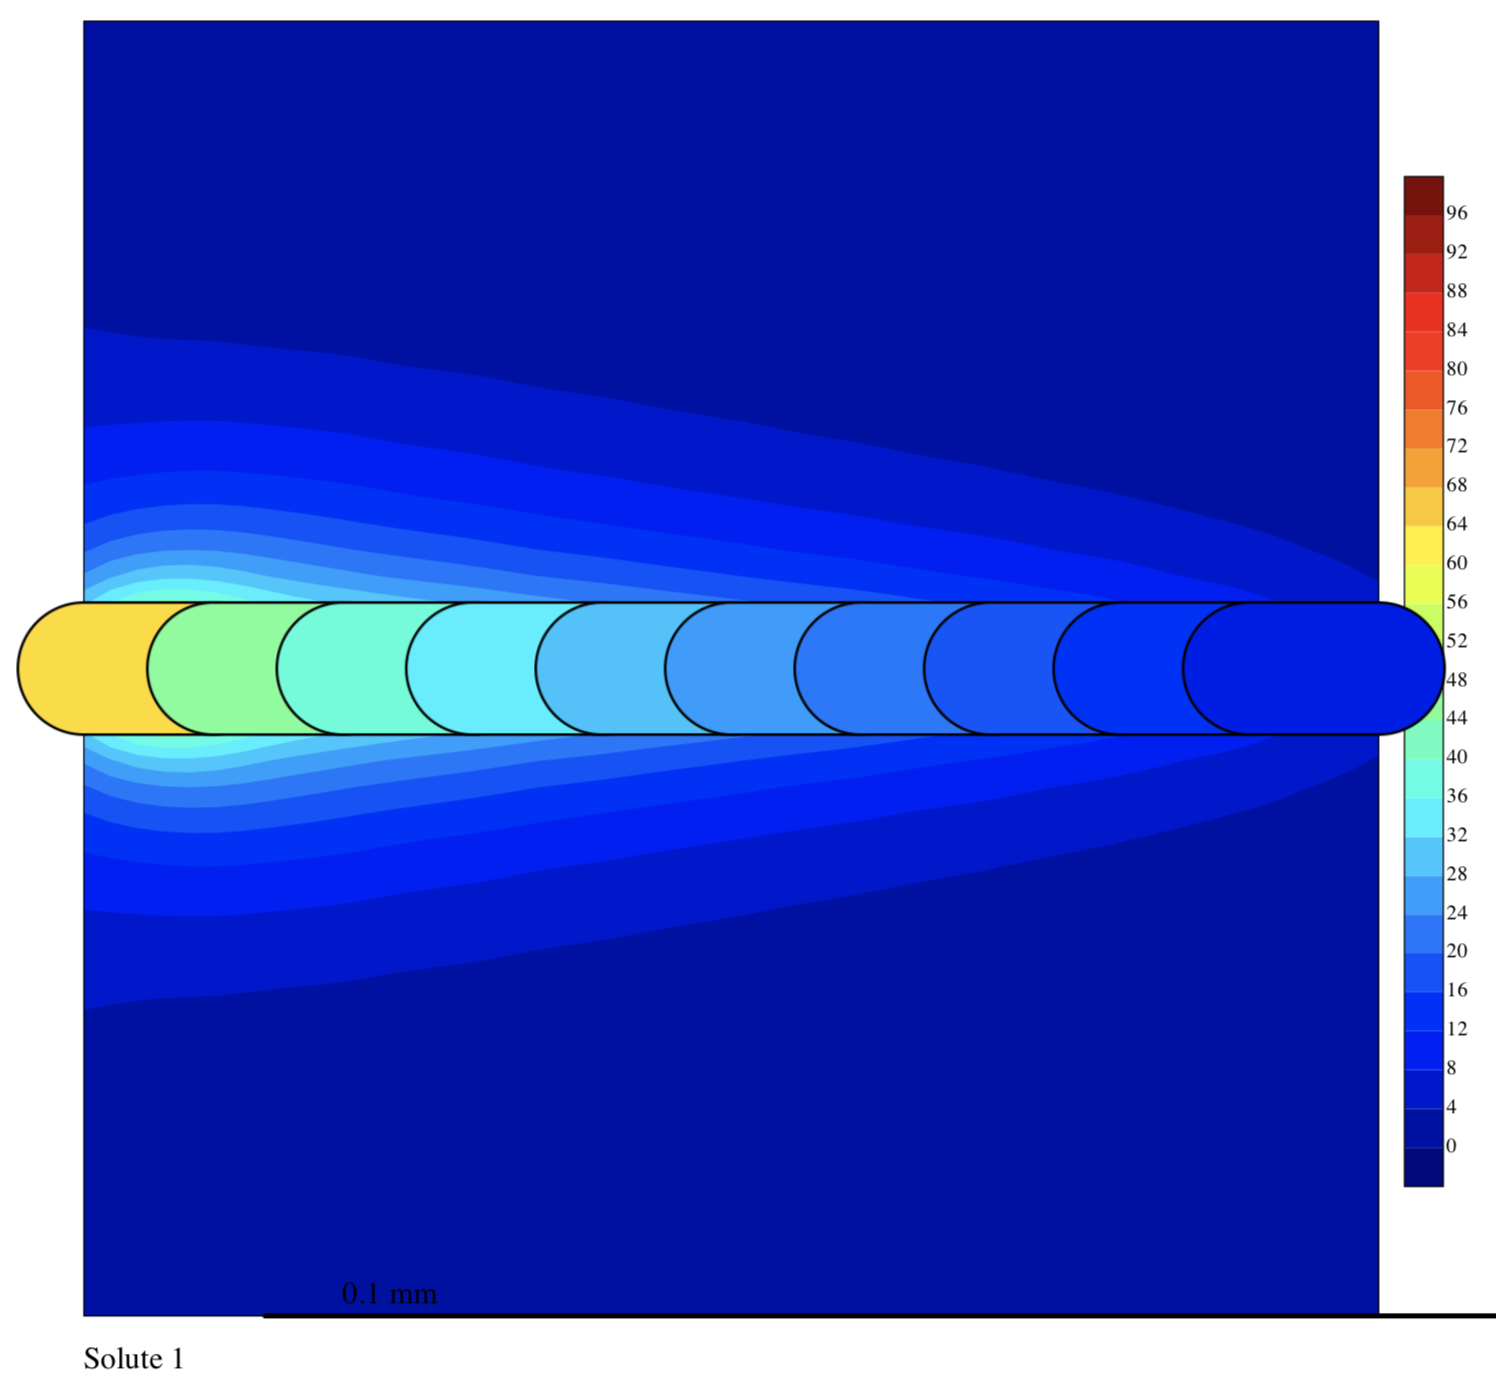
\includegraphics[width=120mm]{Contour_Krogh}
\caption{\footnotesize Green's Contour Output for Krogh Network}
\label{fig:Contour_Krogh}
\end{figure}

%\subsubsection*{Brain Model}
%Explain relevance of this model and the produced results (many plots here)

%The Brain network provided by Secomb (?) was used for further simulations and to validate the produced data.

\subsubsection*{Cardiac Model}
%Explain relevance of this model and the produced results (many plots here)

The Cardiac network provided by Secomb (?) was used for further simulations and to validate the produced data.\\
\\Figure \ref{fig:Contour_Cardiac1}  is the result of a Green's Method blood flow simulation computed on a Cardiac network. The Solute Concentration in the network is visualized.\\
\begin{figure}[h]
\centering
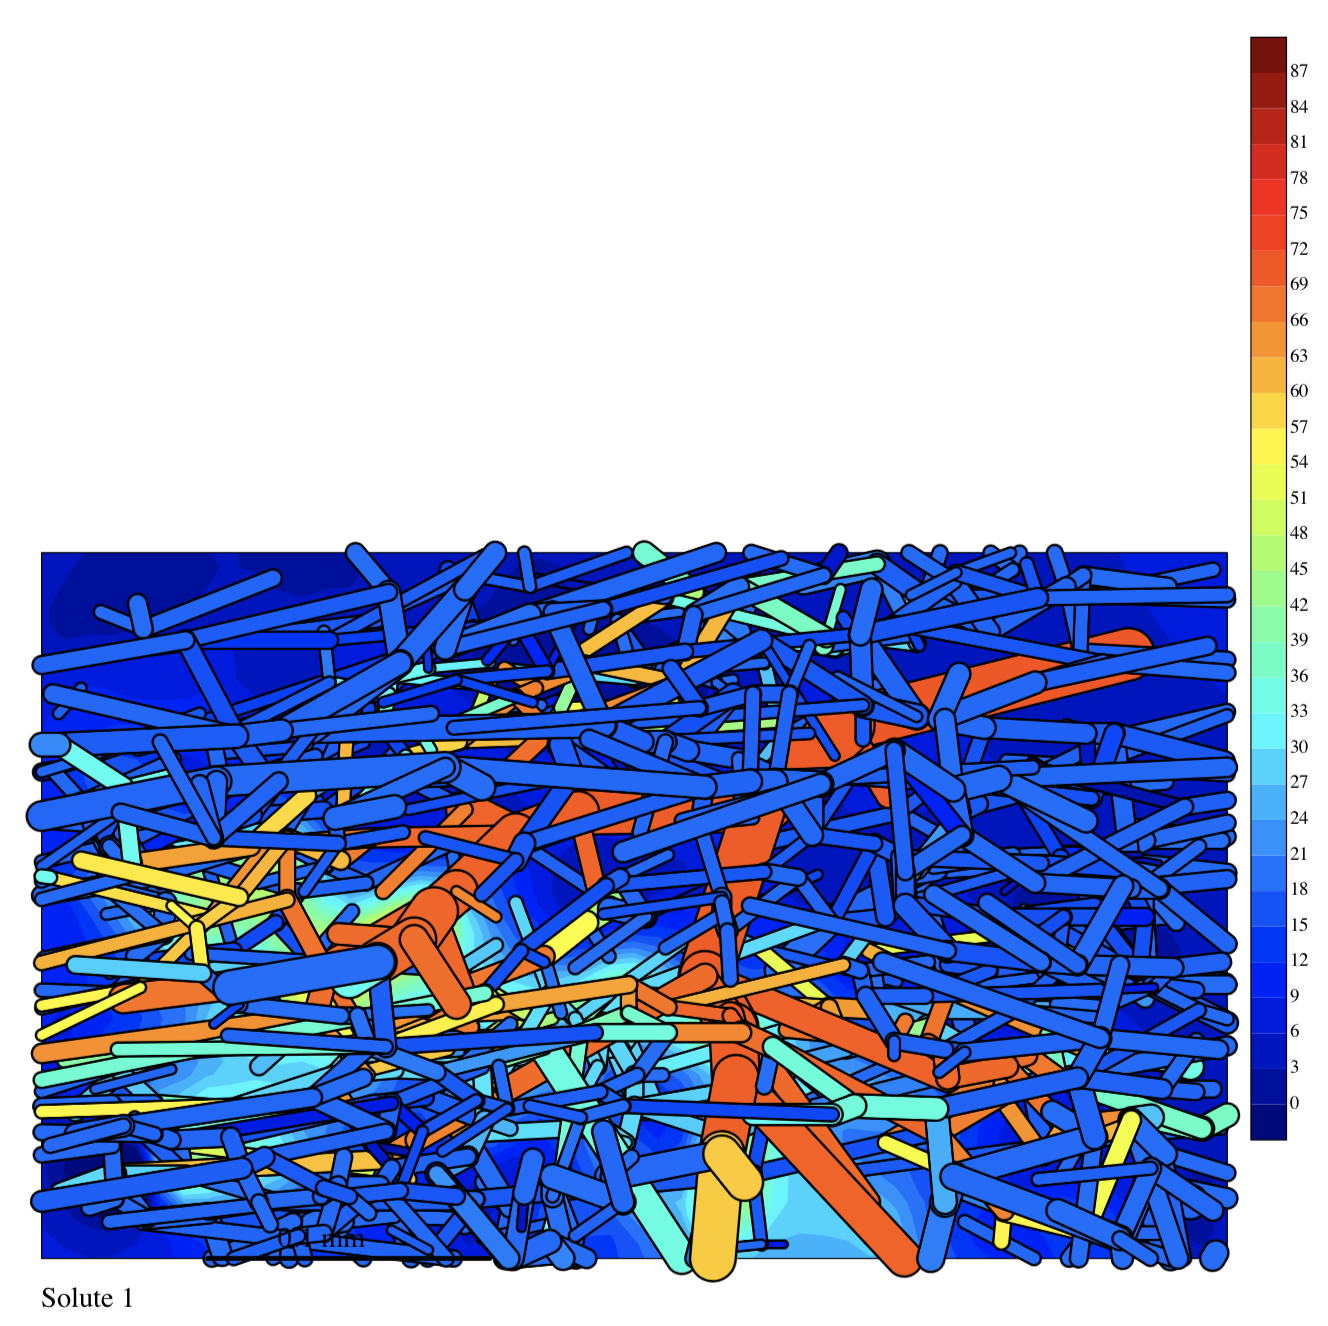
\includegraphics[width=85mm]{Contour_Cardiac}
\caption{\footnotesize Green's Contour Output for Cardiac Network}
\label{fig:Contour_Cardiac1}
\end{figure}

\subsubsection*{Mescent Model}
%Explain relevance of this model and the produced results (many plots here)

The Mescent network provided by Secomb (?) was used for further simulations and to validate the produced data.\\
\\Figure \ref{fig:Contour_Mescent1}  is the result of a Green's Method blood flow simulation computed on a Mescent network. The Solute Concentration of Solute 1 in the network is visualized.\\
\begin{figure}[h]
\centering
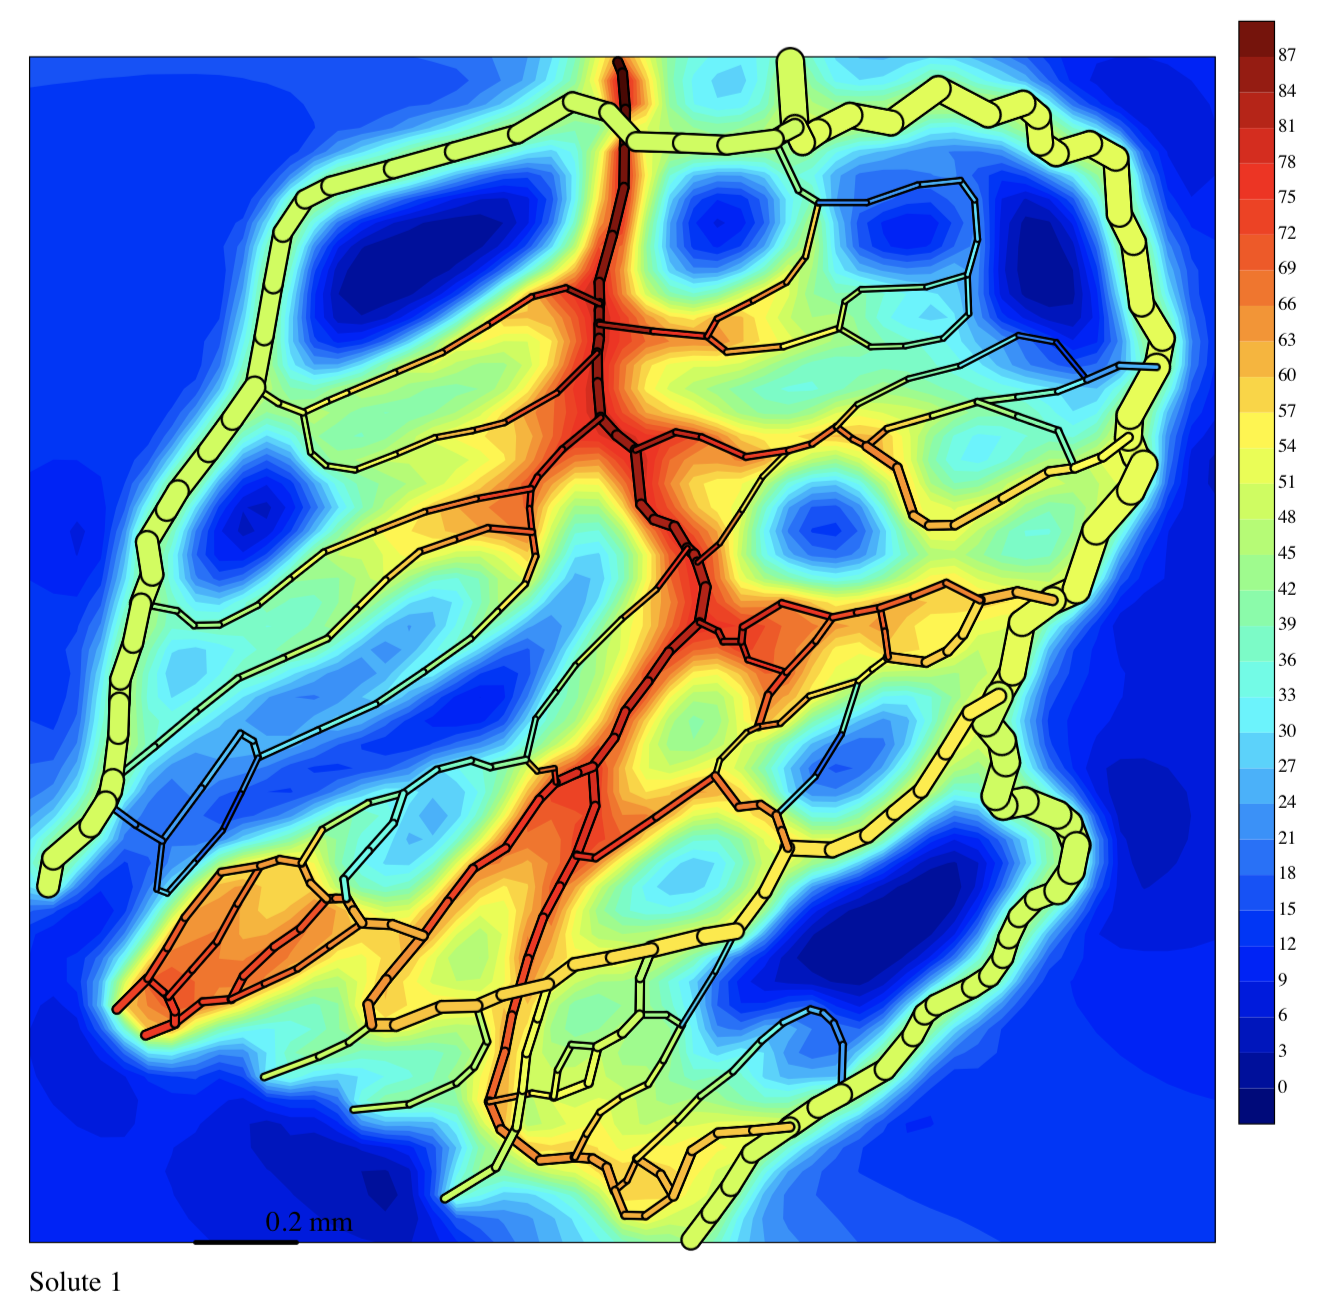
\includegraphics[width=85mm]{Contour_Mescent1}
\caption{\footnotesize Green's Contour Output for Mescent Network (Solute 1)}
\label{fig:Contour_Mescent1}
\end{figure}\\
%
\\Figure \ref{fig:Contour_Mescent2}  is the result of a Green's Method blood flow simulation computed on a Mescent network. The Solute Concentration of Solute 2 in the network is visualized.\\
\begin{figure}[h]
\centering
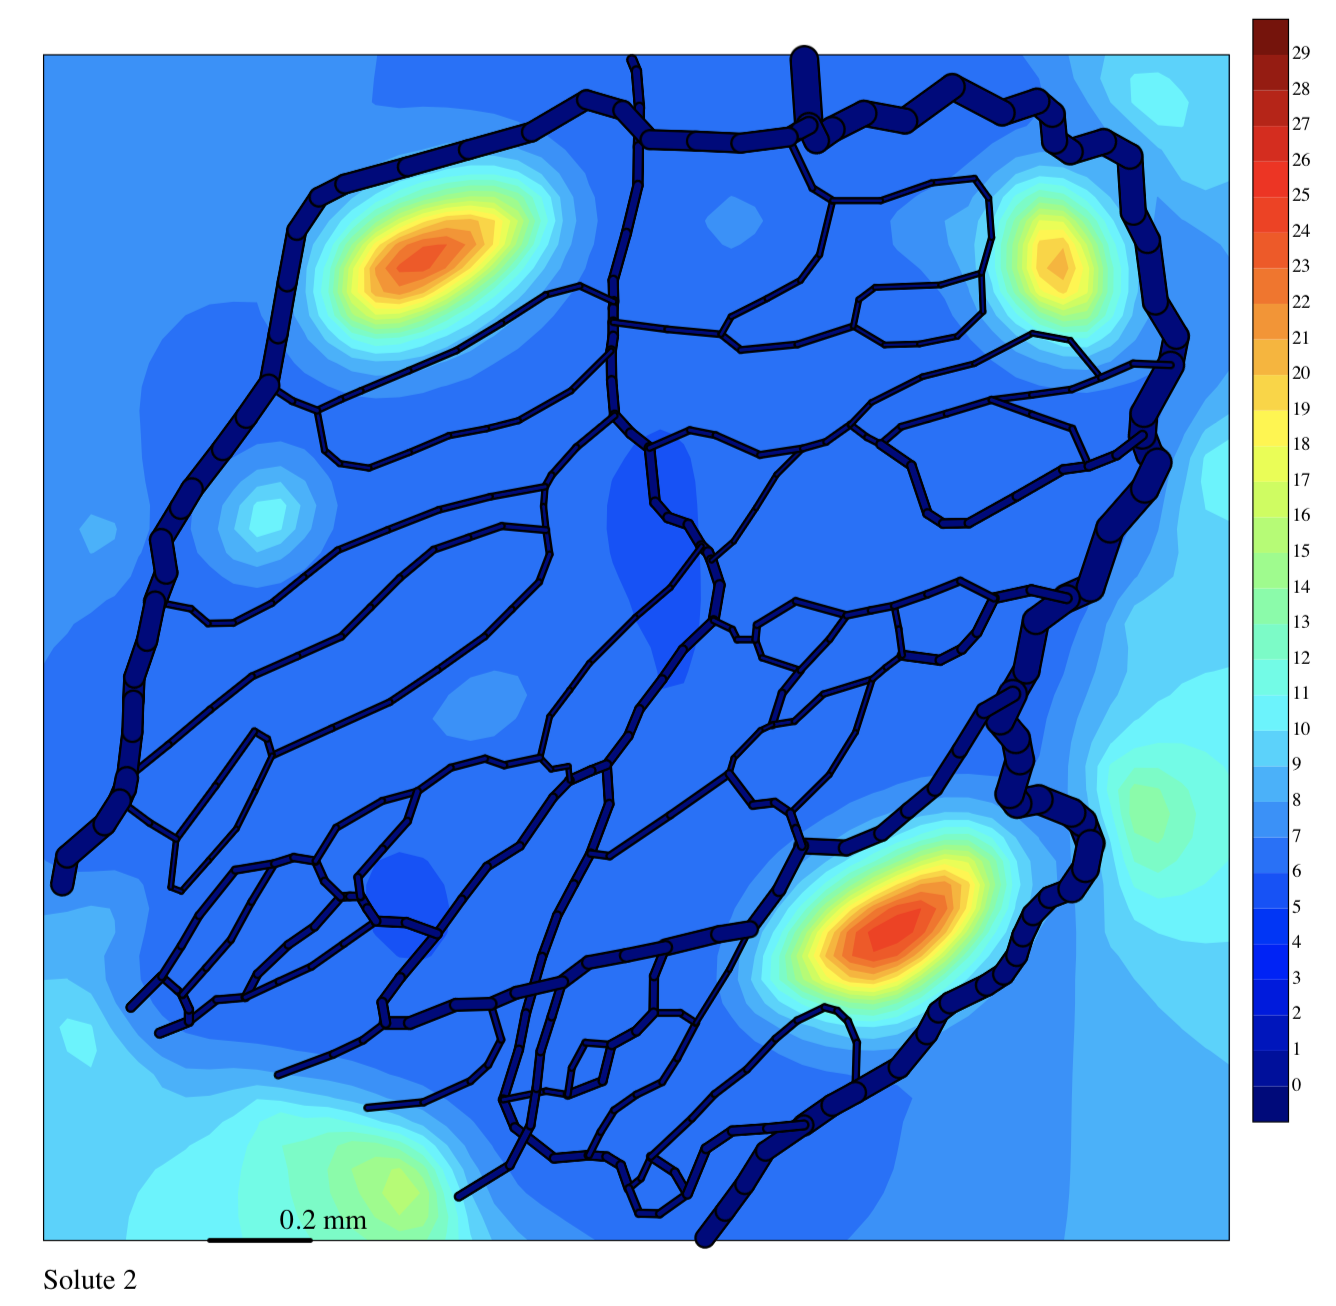
\includegraphics[width=85mm]{Contour_Mescent2}
\caption{\footnotesize Green's Contour Output for Mescent Network (Solute 2)}
\label{fig:Contour_Mescent2}
\end{figure}

\subsubsection*{Tumor Model}
%Explain relevance of this model and the produced results (many plots here)

The Tumor network provided by Secomb (?) was used for further simulations and to validate the produced data.
Figure \ref{fig:Contour_Cardiac1}  is the result of a Green's Method blood flow simulation computed on a Tumor network. The Solute Concentration in the network is visualized.\\
\begin{figure}[h]
\centering
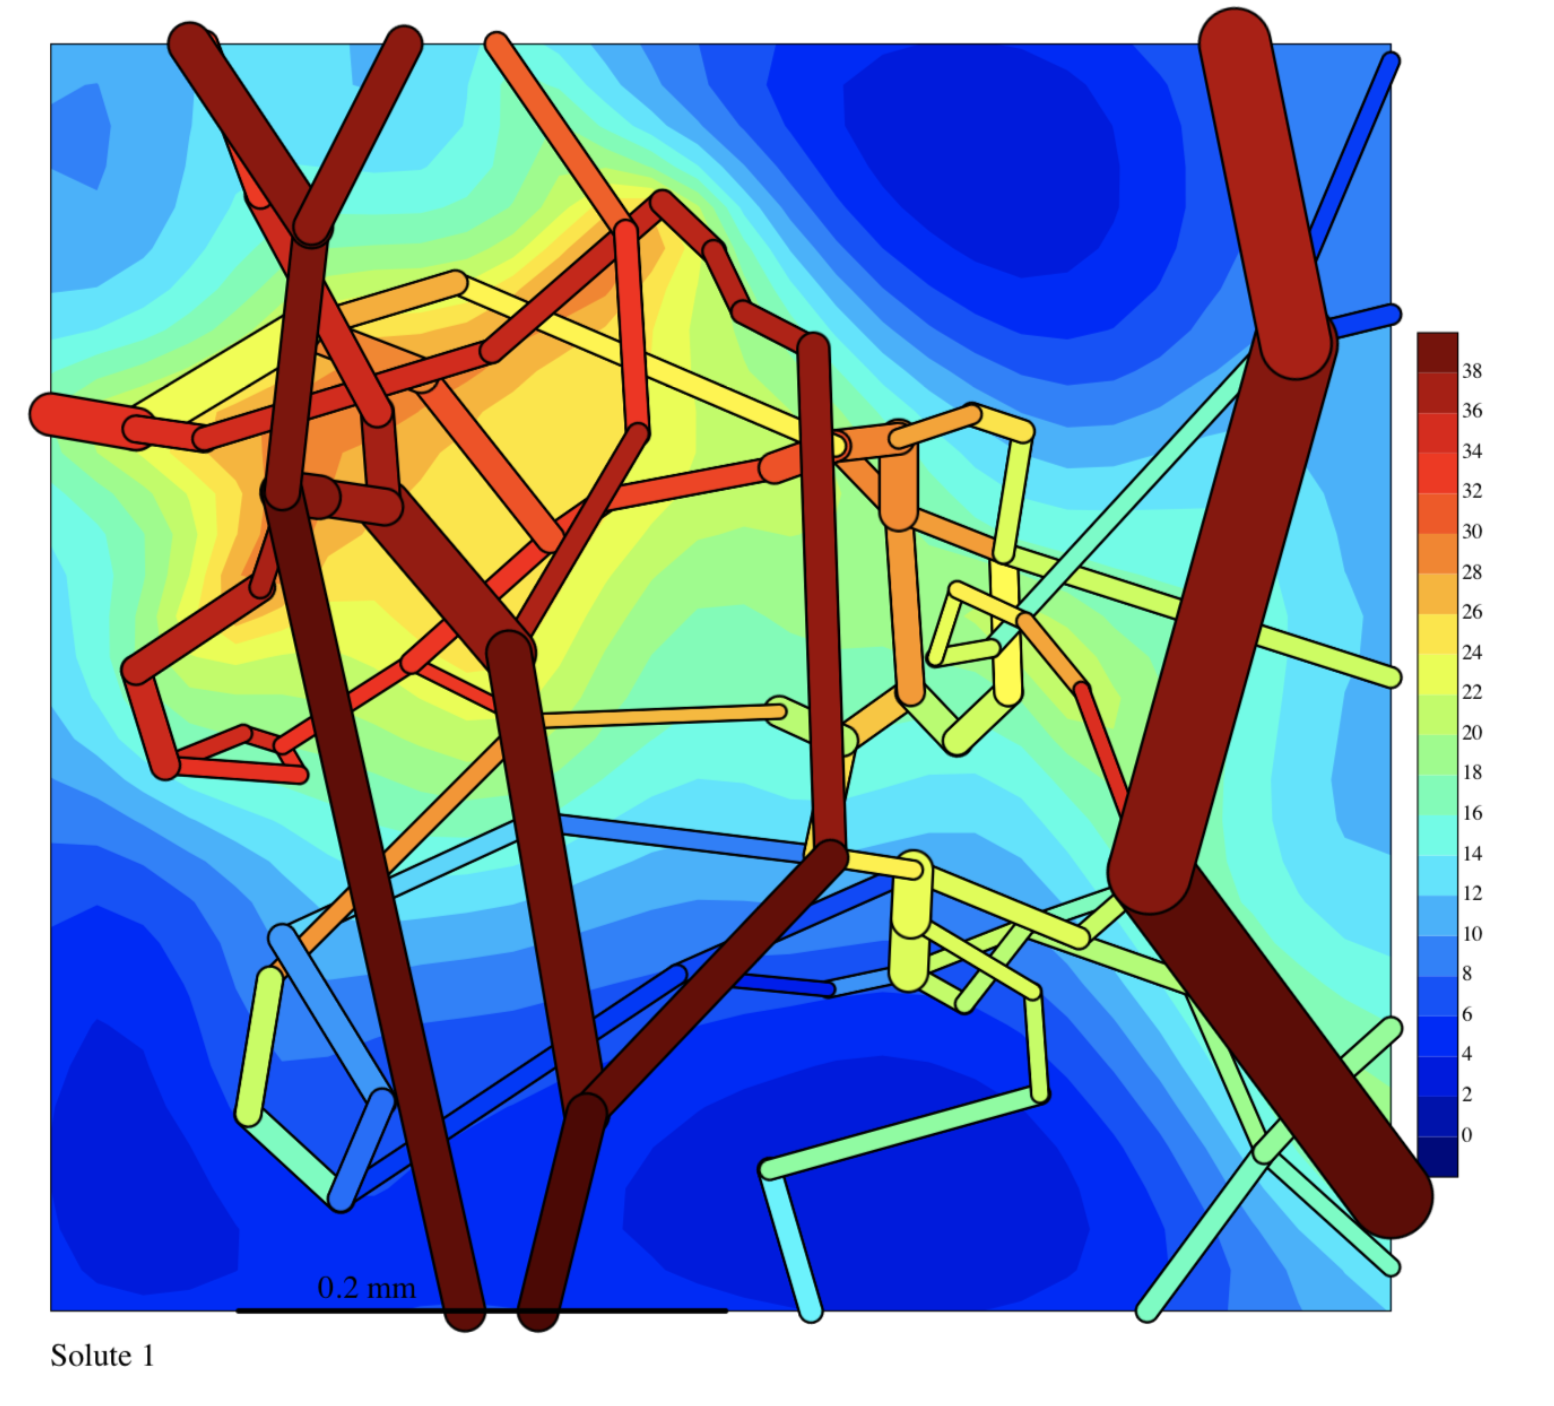
\includegraphics[width=75mm]{Contour_Tumor}
\caption{\footnotesize Green's Contour Output for Tumor Network}
\label{fig:Contour_Tumor}
\end{figure}

\subsubsection*{Further Outlook for New Networks}
%Explain relevance of the new models and the produced results (many plots here)

The results provided by the Green's Method Code were previously discussed for a few networks provided by Secomb (?). In this section the goal is to see how this method can perform in general when it is applied to new networks and to discuss the produced results in detail.

\subsubsection{Discussion of Green's Method and the Produced Results}
%Discussion part of Green's

Final thoughts about Green's Method for physiological applications and oxygen delivery simulations/computations.

\subsection{$DuMu^x$}
%Explain DuMuX in general and explain the implemented method.

$DuMu^x$ is an open source software developed by a strong user community everywhere in the world. The software was basically developed by the University of Stuttgart, and provides a C++ based library of numerical methods and implemented test models, to simulate and solve transport and flow processes in porous media as described in \cite{flemisch2007dumux}.

\subsubsection{General Structure of $DuMu^x$}
%Explain how DuMuX works and what is interesting about it.

$DuMu^x$ is a multi-scale multi-physics toolbox that aims to describe the physical properties of a specific problem as correct as possible, by focussing on minimizing the computational cost \cite{flemisch2007dumux}.\\
\\The structure of $DuMu^x$ is specified in this chapter and illustrated with some figures.
Figure \ref{fig:dumux_structure}  is the Structure of $DuMu^x$ given from the $DuMu^x$ Version 2.12 Documentation \cite{flemischdumux}.\\
\begin{figure}[p]
\centering
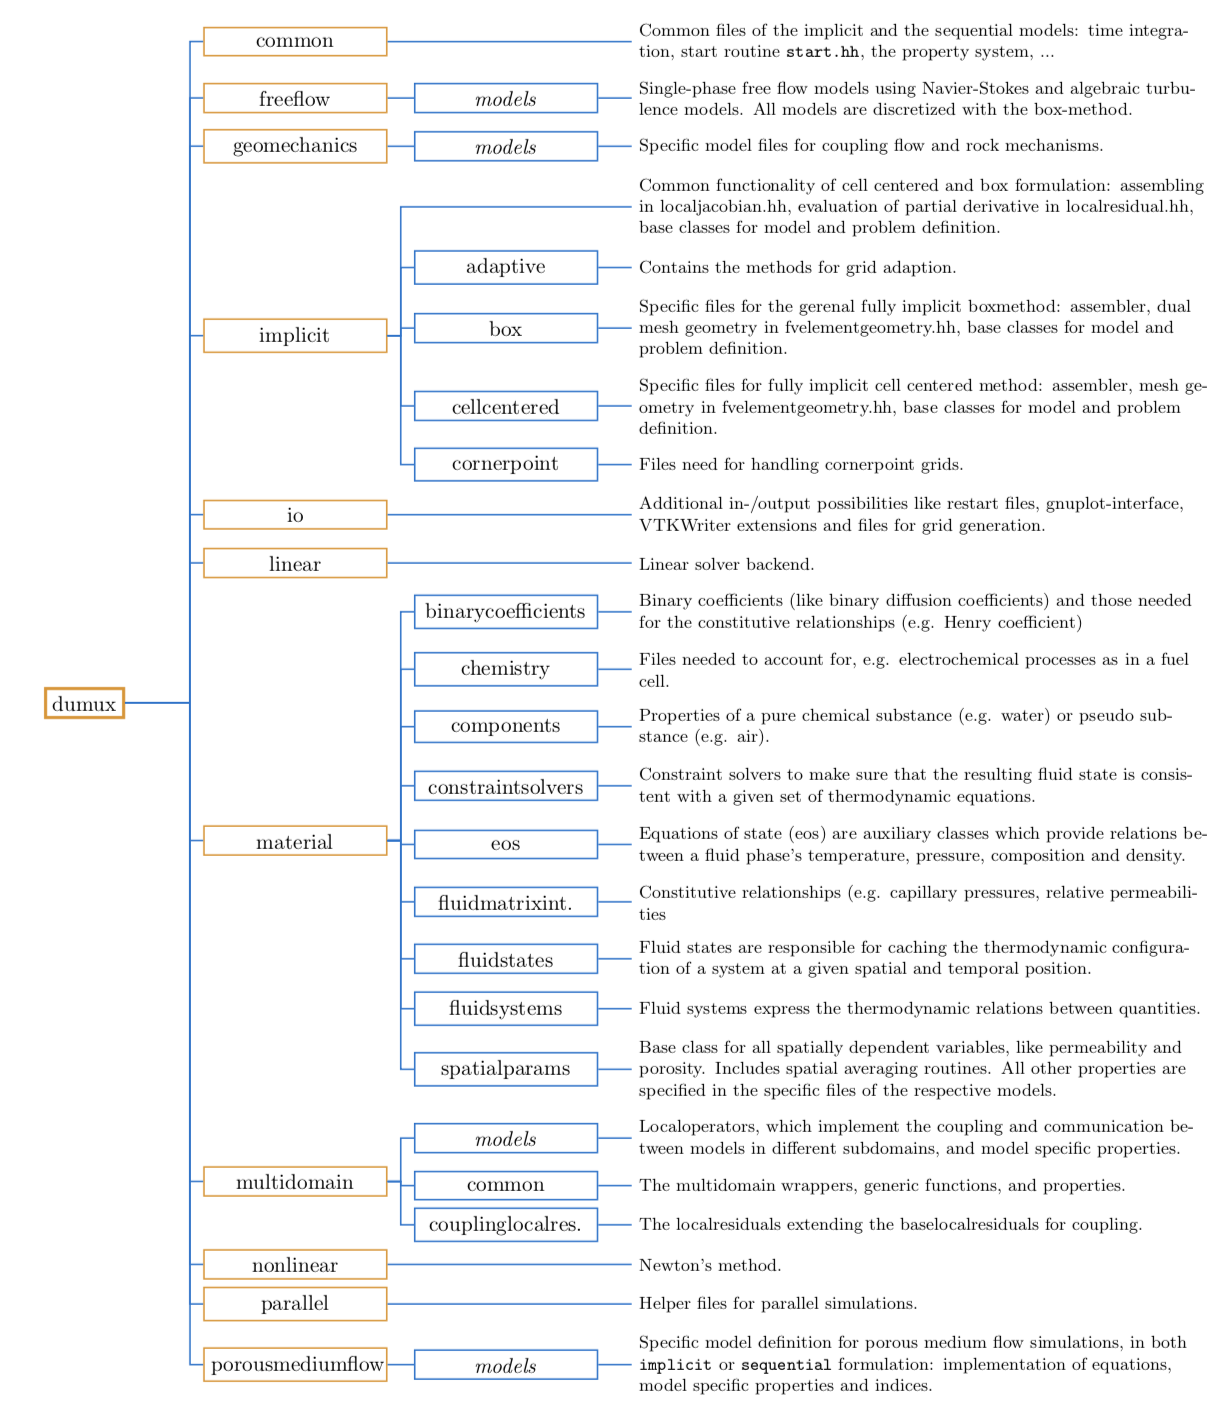
\includegraphics[height=190mm]{dumux_structure}
\caption{\footnotesize The $DuMu^x$ Structure}
\label{fig:dumux_structure}
\end{figure}\\\\\\\\\\\\\\\\\\\\

\subsubsection*{Available Numerical Solvers}
%What solvers can we use ?
%What can DuMuX offer ?

$DuMu^x$ offers a large variety of numerical solvers that be implemented when defining the problem-file. This provides large flexibility in terms of computational cost and stability questions. \cite{flemischdumux}
\\One has to take care to choose a solver that is compatible with the given problem...

\subsubsection{Implemented Model}
%Explain Coupling of Tracer.

While $DuMu^x$ has a modular structure, some of the existing test cases can be combined to solve a more sophisticated and specific problem. In our case, this refers to the coupling of the existing Tracer model to the 1p-1p model. While the 1p-1p model can simulate the flow of a solute in a network by convection and the diffusion of this solute into tissue, the tracer model can literally trace the path of this solute into the tissue, which can be used to obtain oxygen transport and diffusion into the tissue.

\subsubsection*{The 1p-1p Model}
%Briefly explain the 1p_1p Model
%Maybe put some results of the 1p_1p Model here

The 1p-1p model can compute pressure fields and velocities in vessel networks. The velocity outputs can then be used for the tracer model.

\subsubsection*{\footnotesize Some Nephron Network Simulations}

Figure \ref{fig:nephron2_pressure}  is the result of a $DuMu^x$ blood flow simulation computed on a Nephron network. The pressure field in the network is visualized.\\
\begin{figure}[h]
\centering
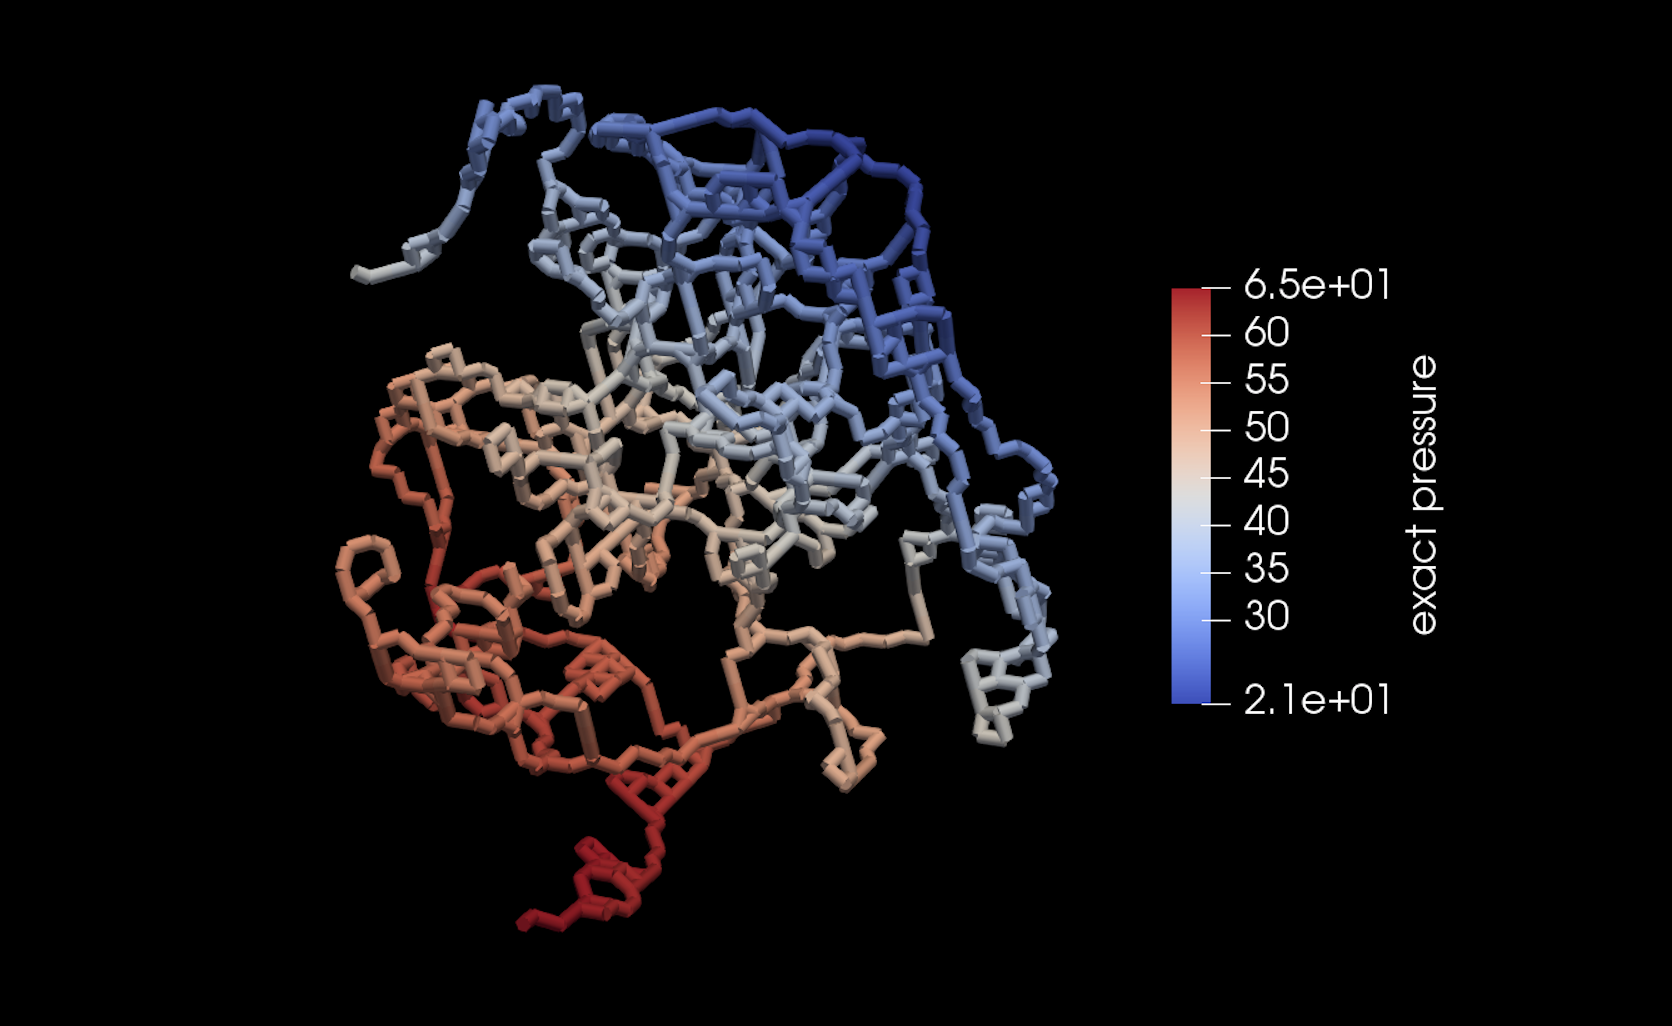
\includegraphics[width=162mm]{nephron2_pressure}
\caption{\footnotesize $DuMu^x$ Pressure Computations for Nephron Network}
\label{fig:nephron2_pressure}
\end{figure}\\
%
\\Figure \ref{fig:nephron2_velocity}  is the result of a $DuMu^x$ blood flow simulation computed on a Nephron network. The velocity field in the network is visualized.\\
\begin{figure}[h]
\centering
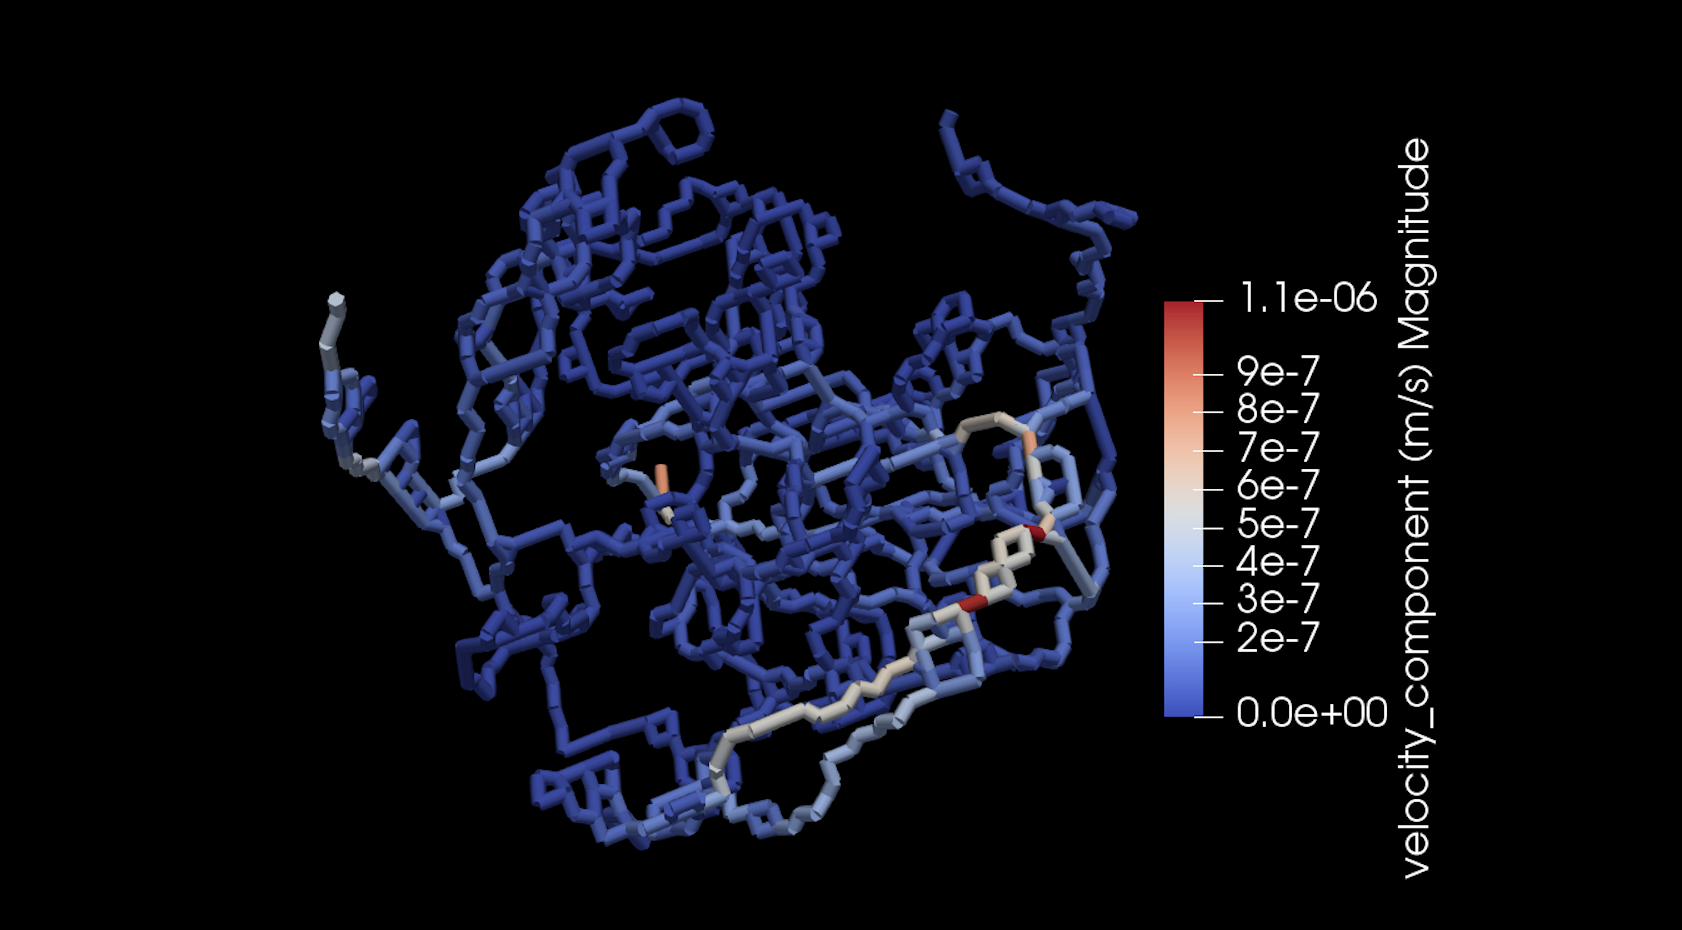
\includegraphics[width=162mm]{nephron2_velocity}
\caption{\footnotesize $DuMu^x$ Velocity Computations for Nephron Network}
\label{fig:nephron2_velocity}
\end{figure}\\\\

\subsubsection*{The Tracer Model}
%Briefly explain the Tracer Model
%Maybe put some results of the Tracer Model here

The tracer model can trace substances in networks and different geometries, and accordingly can compute concentrations/concentration fields of solutes in dynamic systems.
\\This is why I decided to choose the Tracer model to simulate the oxygen transport and diffusion in the given networks...

\subsubsection*{\footnotesize Some Tracer Simulations}

\begin{figure}[h]
\centering
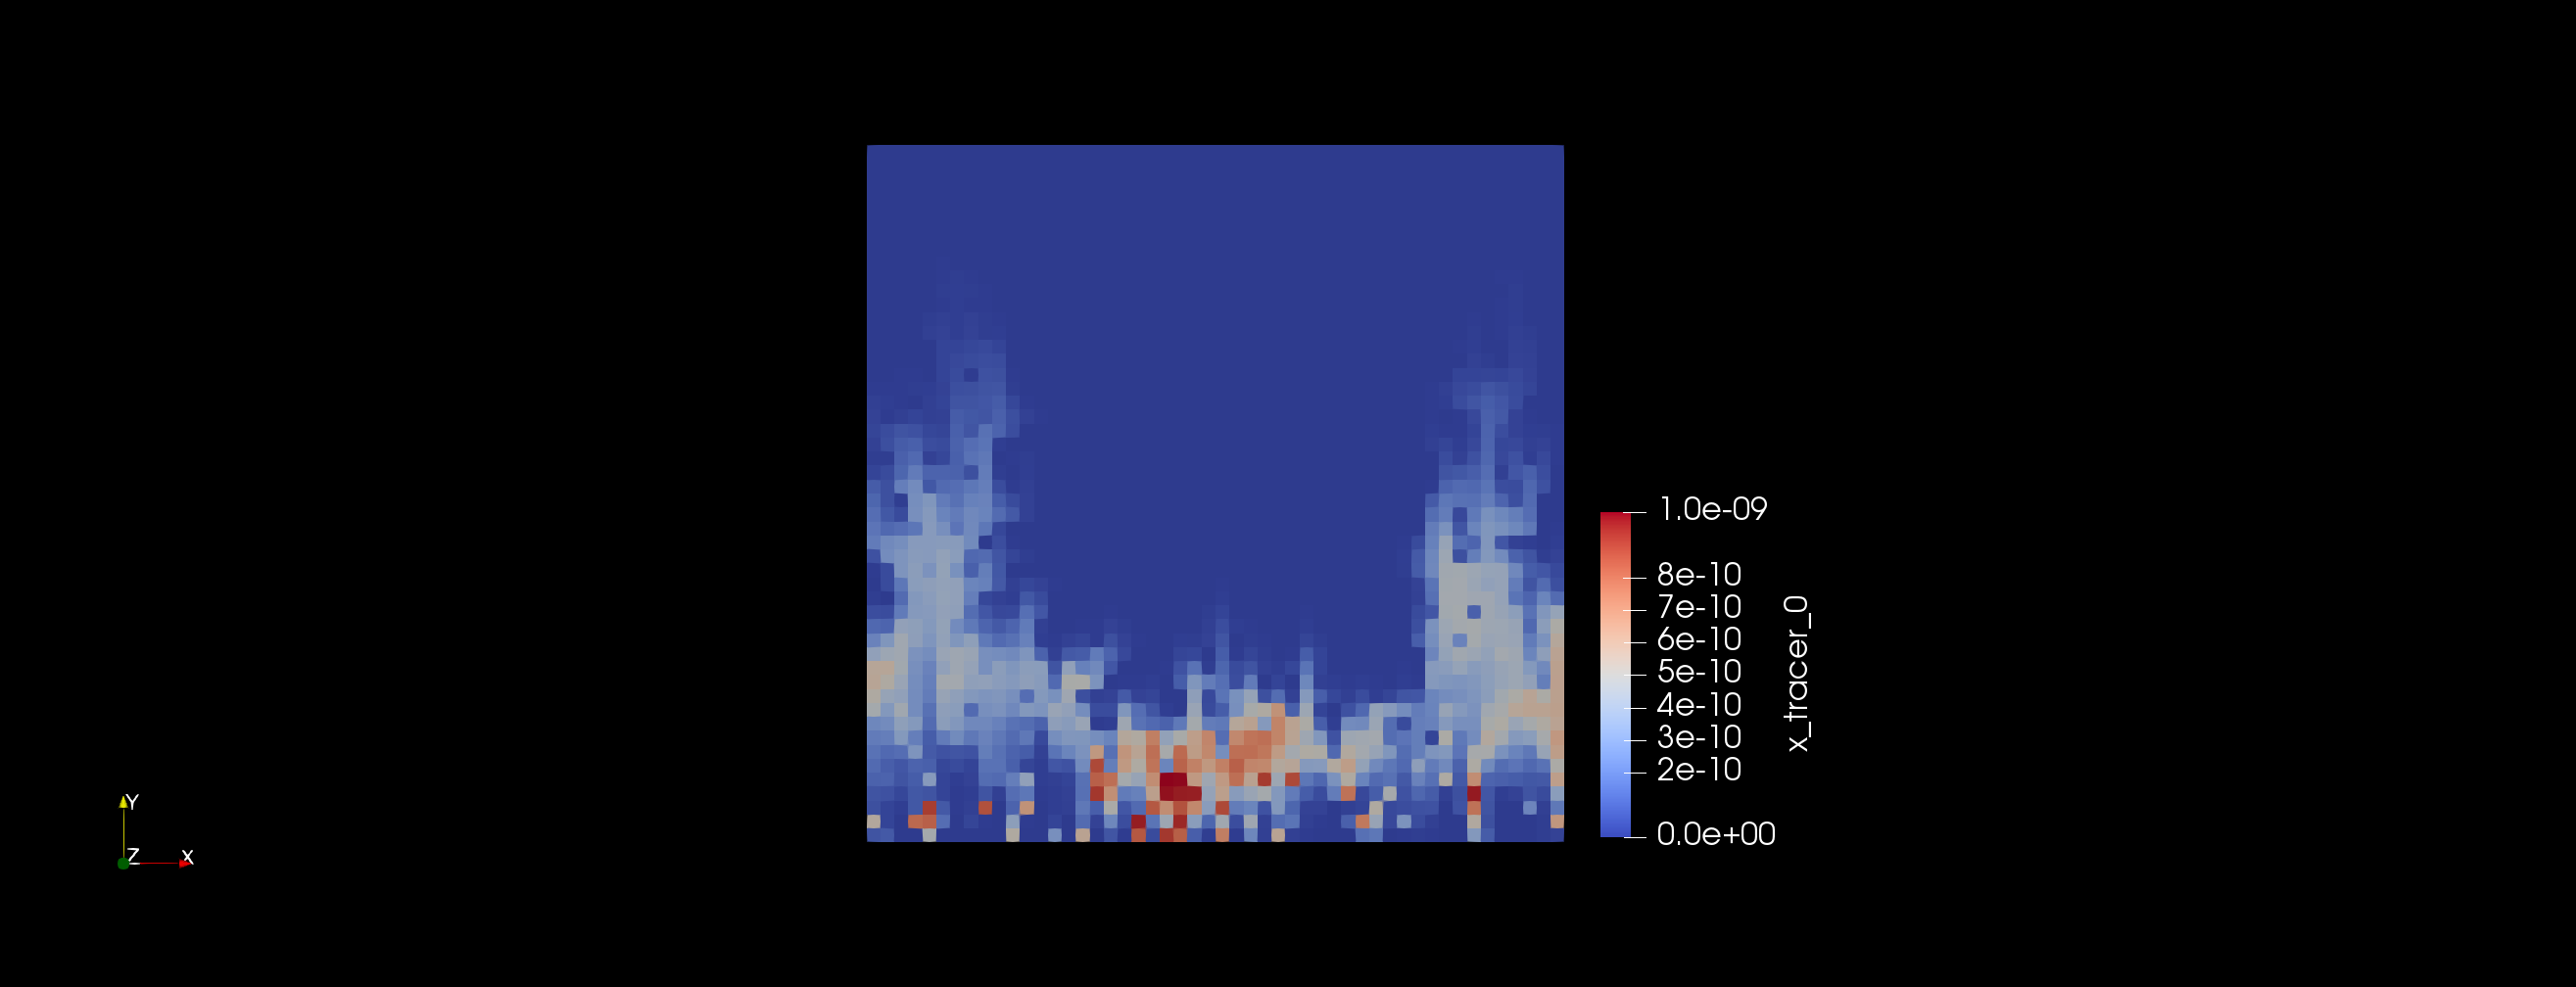
\includegraphics[width=162mm]{tracer_1}
\caption{\footnotesize $DuMu^x$ Tracer Simulation for a Rectangular Geometry}
\label{fig:tracer_1}
\end{figure}
Figure \ref{fig:tracer_1}  is the result of a $DuMu^x$ tracer simulation computed on a rectangular geometry. The solute field in the network for the last time step is visualized.\\

\subsubsection*{The Coupled Model}
%Briefly explain what coupling is and how code is supposed to work
%Hopefully put some results of the coupled model here or explain why the results are wrong

To achieve the goal of tracing oxygen in the given vessel-networks, I coupled the previously described models to obtain a 1p-1p-tracer model...

\subsubsection{Input Data for the Simulations}
%Explain where the networks come from: CT by Willy and Artery/Vein recognition by Diego

The networks that were used for the simulations are extracted from real organs coming from mice. This process is done by scientists from different areas of expertise and is usually performed in the following order:
\\1)CT of the kidneys
\\2)Recognition of fat, tissue, arteries and veins by machine learning algorithms
\\3)Three dimensional captions of the organ are build by many virtual two dimensional slices
\\4)Transformation of the recognized artery/vein data into networks that can be used for the simulations.

\subsubsection{Results}
%Results part of DuMuX
-Pros/Cons
\\-Quality of results
\\-Paraview Visualization of results

\subsubsection*{Some Nord Network Simulations}
%I will hopefully put 1p_1p_tracer results here later

Figure \ref{fig:nord_pressure}  is the result of a $DuMu^x$ blood flow simulation computed on a Nord network. The pressure field in the network is visualized.\\
\begin{figure}[h]
\centering
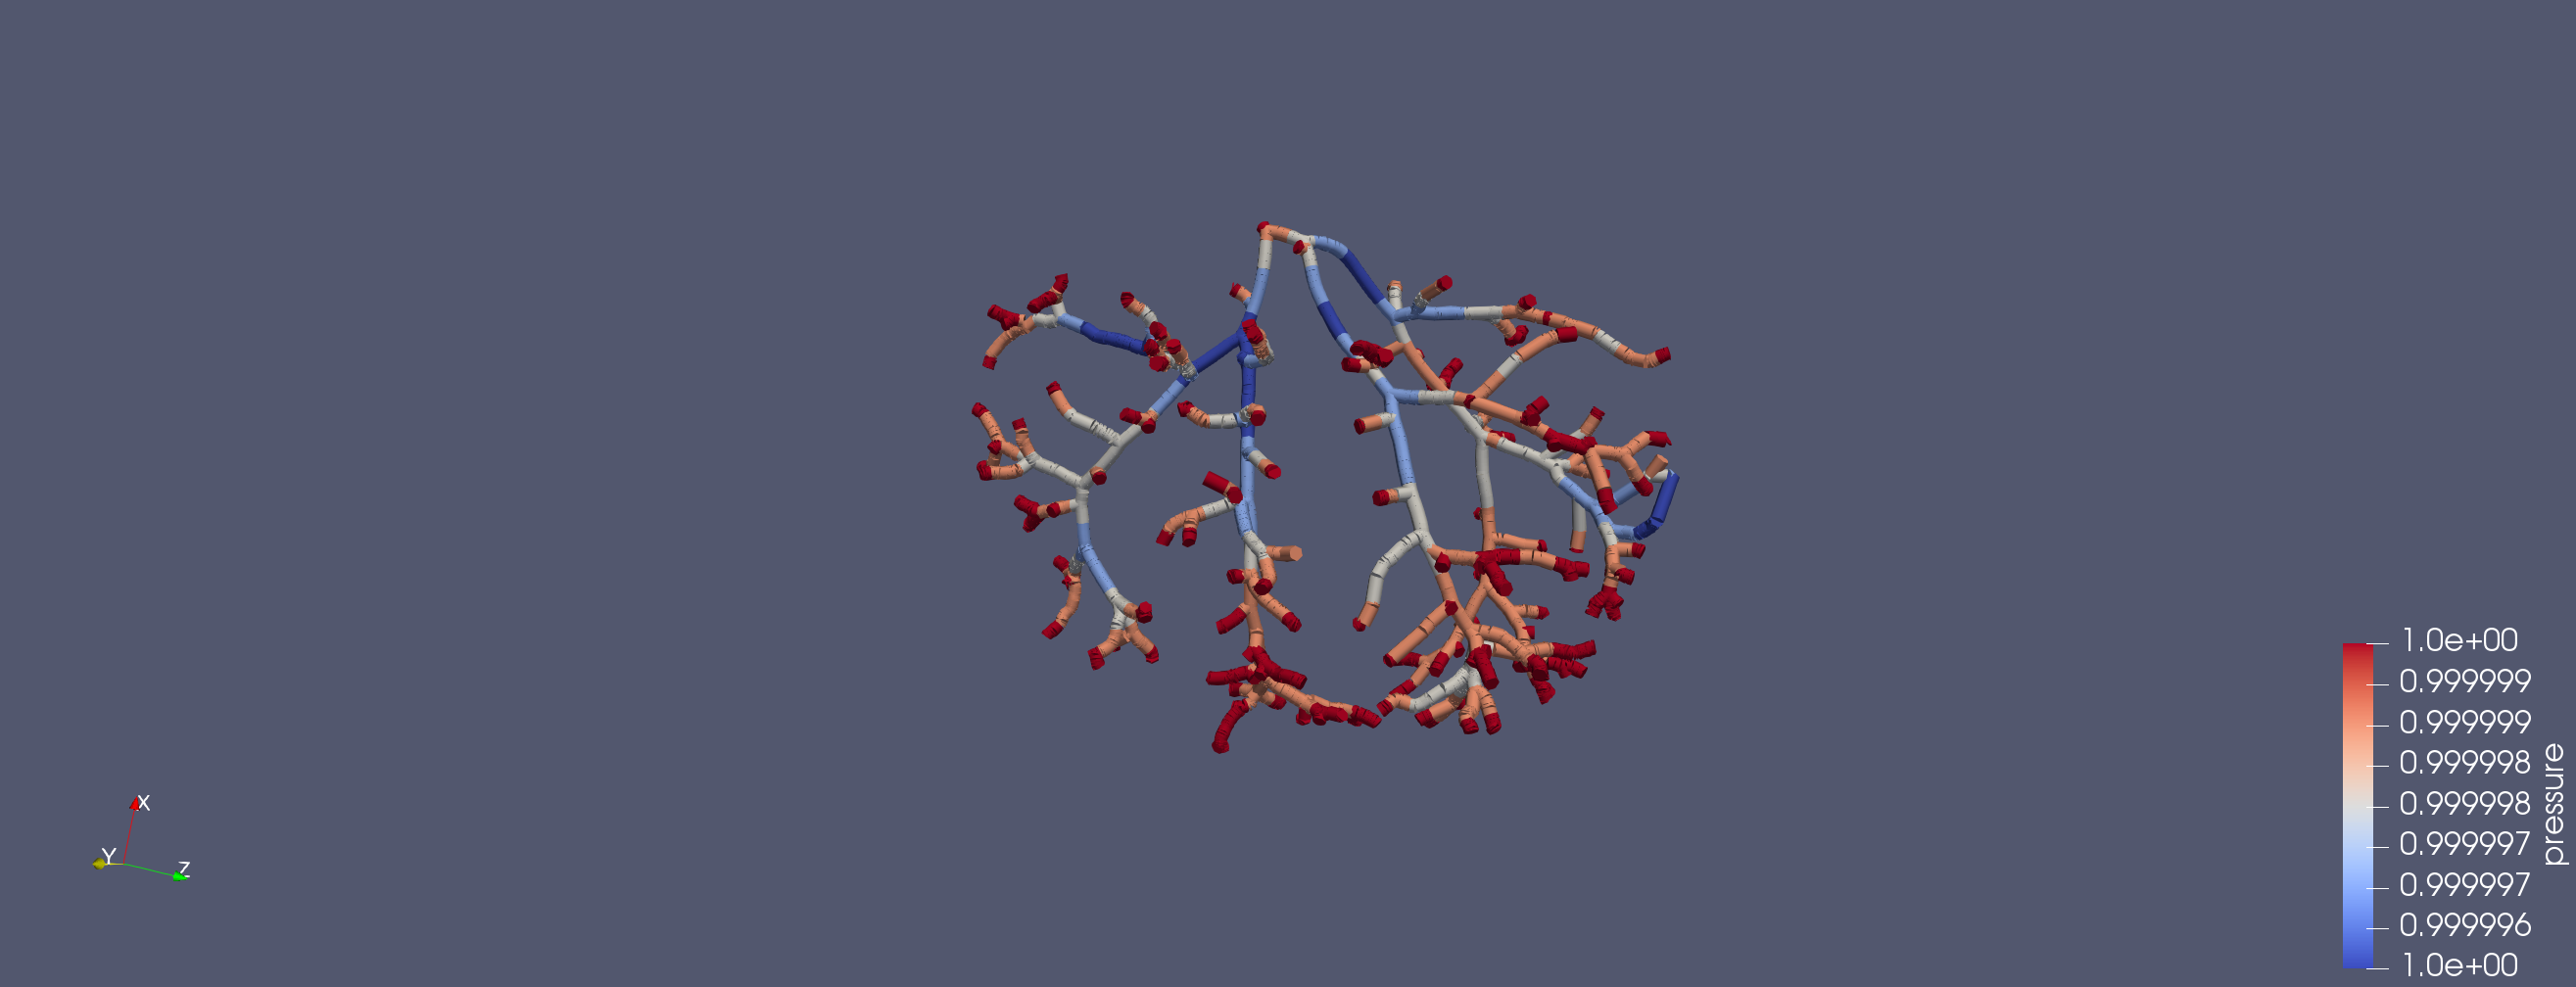
\includegraphics[width=162mm]{nord_pressure}
\caption{\footnotesize $DuMu^x$ Pressure Computations for Nord Network}
\label{fig:nord_pressure}
\end{figure}\\\\
%
\\Figure \ref{fig:nord_velocity}  is the result of a $DuMu^x$ blood flow simulation computed on a Nord network. The velocity field in the network is visualized.\\
\begin{figure}[h]
\centering
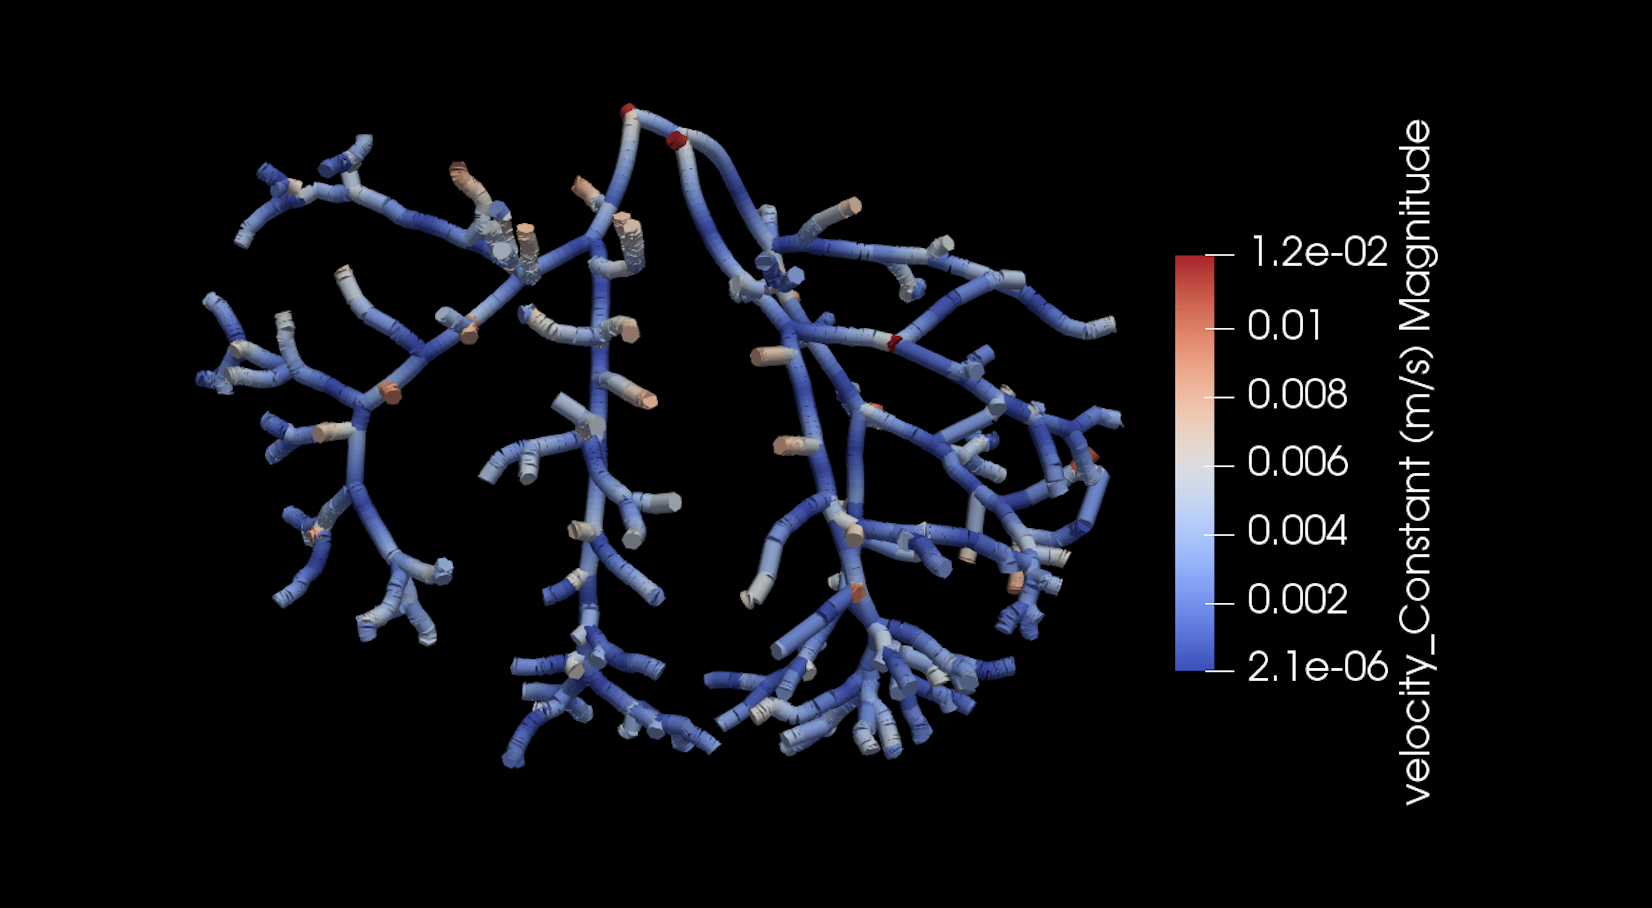
\includegraphics[width=162mm]{nord_velocity}
\caption{\footnotesize $DuMu^x$ Velocity Computations for Nord Network}
\label{fig:nord_velocity}
\end{figure}\\\\

\section{Comparison of the Different Methods Behind the Simulations}
%Compare DuMuX to Green's Method in general
In this section the main differences between these two simulation methods described previously will be discussed.

\subsection{Comparison of the Methods}
%Compare the Solvers behind the Methods
%Very useful tu use Secomb Paper Numerical Methods section here
In this section the main differences between the solvers and the associated numerical methods will be discussed.
\\
\\As mentioned previously, one of the huge advantages of $DuMu^x$ is the flexibility it provides in terms of solvers, and thus in terms of the numerical methods used for the computations. This means that it is often possible to pick a solver which is stable for the specific problem and the chosen discretization.
\\
\\This is obviously different for the Green's Method code, as there is no option of choosing a different solver than the one provided in the code. As discussed previously, this code is specifically implemented to solve and compute oxygen (or other Solute) concentrations in the blood and the surrounding tissue, and the implemented method strongly relies on the stability of the Green's Method and the numerical methods behind the solver.

\subsubsection{Comparison of the Numerical Methods}
%Explain the Methods and differences between methods
%Very useful tu use Secomb Paper Numerical Methods section here
In this section, the focus will be on comparing the numerical methods behind the Green's Method code and $DuMu^x$ and the differences in their implementation.

\subsubsection{Stability Questions and Computational Cost}
%Explain when and why which the numerical methods are stable
In this section, the consequences of the previously described differences will be discussed. The focus lies on the differences in terms of stability and computational cost for similar simulations.

\subsection{Comparison of the Results}
%Compare the produced results
In this section the main differences in the produced results for the same input files/same networks will be discussed.

%\section{Discussion}

%I already did this previously, so might delete this part ...

\section{Conclusion}
%Summary of both methods in general and Outlook for the research field
%What this review was about: short summary. Main points
%highlighted. Perhaps a graph regrouping together elements.
%Comparison of different strategies and their state. Maybe your own
%thoughts on the whole story and where the promising directions lie
%and which ones you see with scepticism.

As seen previously, both the Green's Function Method and the implemented $DuMu^x$-based method can offer very interesting options. While the Green's Function Method is presenting a specifically created C++ based software for oxygen Transport and Diffusion simulations, the results show that the obtained outputs are not always satisfying (eventually will happen for new networks?). The reasons for this have been discussed previously (maybe repeat them shortly here).
Compared to this, the $DuMu^x$ based model is still in its very initial phase and cannot produce correct results yet (very probably). Still, the fact that it is $DuMu^x$ based offers both a large flexibility to the user in terms of further development, as well as in terms of computational flexibility when choosing a time- and space-discretization through choosing discretization modules and different grid creators. The solvers can also be chosen by the user, which doesn't guarantee an overall stable numerical solver, but can provide great flexibility when adapting the model to specific networks.
\\
\\Main conclusions and final remarks.


\section{Acknowledgements}
Thank you all for the support blabla...